%!TEX root = ../rapport.tex

\chapter{Look of the Graph Drawings}

In this Chapter we present the thoughts on the look of the generated drawings
and the decisions we made concerning colouring, sizing, etc.

\section{Direction}

The graphs are directed, so some kind of arrow heads need to be drawn. Since
an edge can be drawn spanning a lot of screen area, the type of arrow has to
be designed such that it is clear to see where an edge starts from the arrow
head alone and vice versa. An alternative to arrows is drawing the edges with
a colour gradient. In this approach, an edge would be couloured e.g. green at
the start and red at the end, interpolating the colours on the edge line. 

A study of the usability of these and other methods is presented in
\cite{Holten2009}. In this study, the representation that performed best was
the so-called ``tapered'' representation, ``[...] in which the width of an
edge is gradually varied along its length -- wide at the start and narrow at
the end [...]'' \cite[p. 2307]{Holten2009}. The authors recommend avoiding the
intuitive representation, where a ``normal'' arrowhead is drawn, altogether.
Nonetheless, for our purposes, we found that the regular arrow heads gave
reasonable results, and they have the benefit that they are easy to implement.
In a future version of the software alternatives to this approach could be
explored.

\section{Edge Weighting}

As seen in Chapter \ref{chap:theory} there can be more than one edge between
two nodes in a $\beta$-reduction graph. We have chosen not to display this
information and instead draw each connection between nodes for terms $M$ and
$N$ as a single line, regardless of whether there are one or several ways to
reach term $N$ from term $M$. This is done in an effort to reduce the visual
clutter in the drawing; for terms with e.g. 10 redexes that all have the same
constractum it would be distracting to see 10 lines on the drawing, all of
them between the same two nodes. For instance, the term $M_{K_{10}}$ below has
several redexes that all have the same contractum, $y$:
\begin{equation*}
	M_{K_{10}} \equiv
	(\lam{x_1}{y}) 
	((\lam{x_2}{y}) 
	((\lam{x_3}{y}) 
	((\lam{x_4}{y}) 
	((\lam{x_5}{y}) 
	((\lam{x_6}{y})
	((\lam{x_7}{y})
	((\lam{x_8}{y})
	((\lam{x_9}{y})
	(\lam{x_{10}}{y}))))))))) \barrow y
\end{equation*}
An alternative would be to annotate each line with its ``weight'', i.e. write
``10'' on the line. However, in a drawing of a reduction graph with e.g. 50
edges lying in close proximity to each other, these numbers could easily get
mixed up.
\begin{figure}[htbp]
	% (#x1.(y)) ((#x2.(y)) ((#x3.(y)) ((#x4.(y)) ((#x5.(y)) ((#x6.(y)) ((#x7.(y)) ((#x8.(y)) ((#x9.(y)) ((#x10.(y)))))))))))
	\centering
		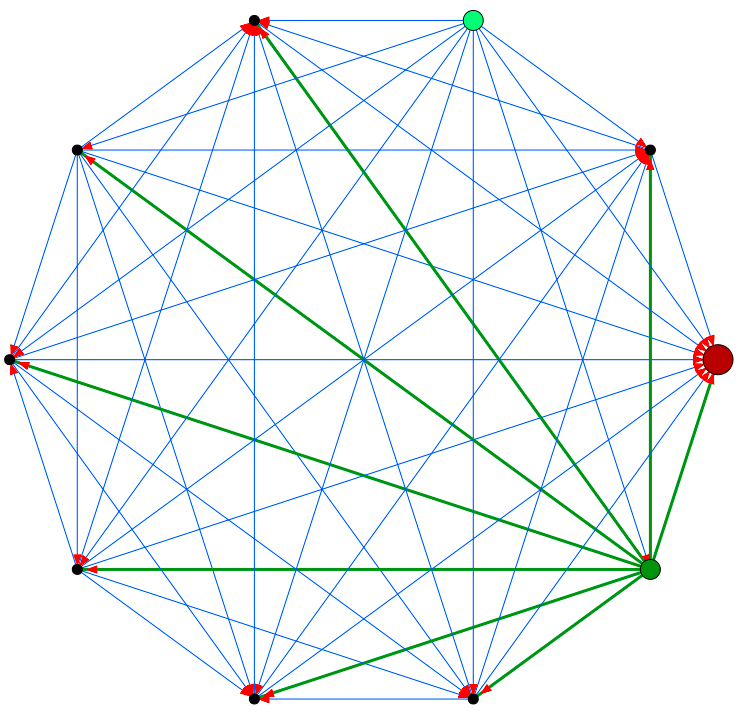
\includegraphics[height=2in]{../images/lambda_k10_CIRCO.png}
	\caption
	[$M_{K_{10}}$, a reduction graph version of $K_{10}$.]
	{$G_\beta(M_{K_{10}})$, drawn with the Circo algorithm.}
	\label{fig:images_lambda_k10_CIRCO}
\end{figure}

\section{Colouring}

To be able to distinguish between different kinds of nodes in the reduction graph,
different variants of colouring and sizing are used:
\begin{itemize}
	\item The normal form, if any, must be easily recognizable. Therefore it is
	coloured red and drawn as the biggest node: 
\includegraphics[height=0.2in]{../images/NF_example.png}.
	
	\item The start term is represented by a light green, medium sized node: 
	
\includegraphics[height=0.12in]{../images/STARTNODE_example.png}.
	This makes it easy to recognize
	
	\item The current term that is being ``expanded'', that is, having all its
	redexes reduced to their contracta, is coloured dark green and made medium size:
	
\includegraphics[height=0.12in]{../images/CURRENTNODE_example.png}.
	Also, all the edges representing reductions are drawn thicker than the other edges
	and in the same dark green colour as the node.
	
	\item Regular nodes in the reduction graph are drawn as small, black dots.
	Edges representing reduction that are not the ``current'' reduction are
	drawn as thin, blue lines.
	
	\item All self-referencing nodes, i.e. nodes with an edge that is both outgoing 
	and ingoing, are drawn as red squares: 
\includegraphics[height=0.1in]{../images/redsquare_example.png} . 
	If the start term is self-referencing,
	it is drawn as a light green, medium sized circle with a red square inside.
	
	\item The arrow heads on the edges are bright red, making them easily 
	distinguishable in a cluttered drawing.
	
	\item To make it easier to quickly see where the contracta of a given node are,
	all its outgoing edges are highlighted by being drawn with thicker lines
	when it is clicked, see Figure \ref{fig:images_highlighted_node_DOT}. 
	This only happens if the node has been expanded. Only one node can have 
	its edges highlighted at a time, so all previously highlighted edges are 
	reverted to their normal look if a new node is clicked. 
\end{itemize}
\begin{figure}[htbp]
	% #B1.((((#B2.(#B3.(#B4.(B2))) (#B5.(#B6.(#B7.(#B8.(B1)))) #B9.((#B10.((#B11.(B9) #B12.(#B13.(#B14.(#B15.(B1)))))) #B16.(F1))))) #B17.(B1)) #B18.((#B19.(#B20.(B19)) (#B21.(B21) ((B1 #B22.(#B23.(B22))) #B24.(#B25.(#B26.((#B27.(B25) B25))))))))))
	\centering
	\subfigure[Drawn with the Dot algorithm.]{
		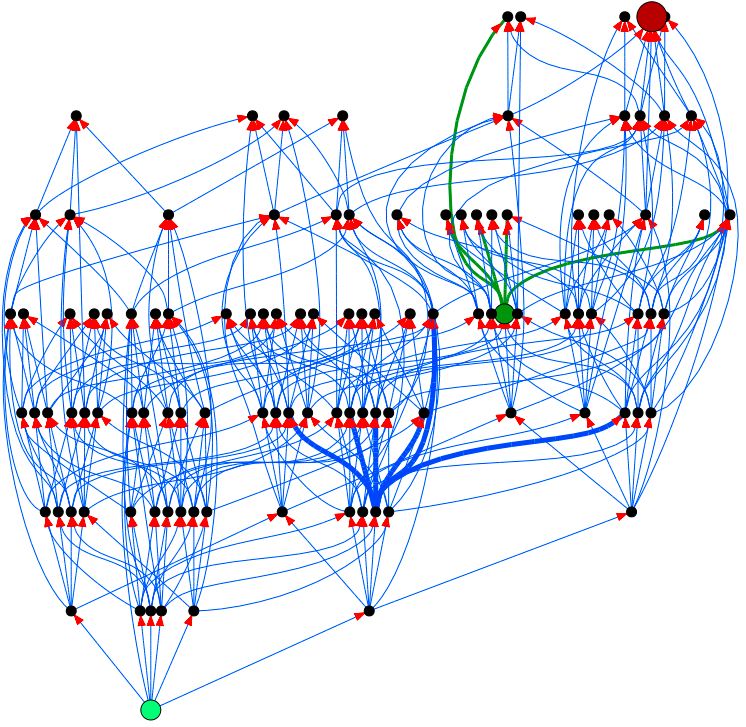
\includegraphics[height=2.5in]{../images/highlighted_node_DOT.png}
	}
	\subfigure[Drawn with the Neato algorithm.]{
		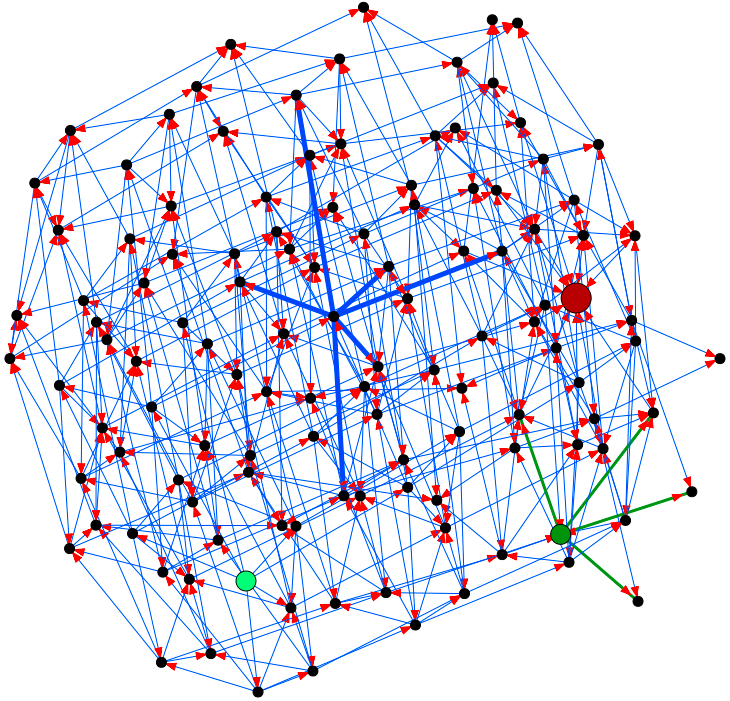
\includegraphics[height=2.5in]{../images/highlighted_node_NEATO.png}
	}
	\caption
	[Complex, 27-abstractor lambda term.]
	{A complex lambda term with 27 abstractors with a node and its outgoing
	edges highlighted.}
	\label{fig:images_highlighted_node_DOT}
\end{figure}
